\documentclass[11pt,letterpaper]{article}
\usepackage{amsmath,amssymb,amsthm}
\usepackage{graphicx}
\usepackage[margin=0.6in]{geometry}
\usepackage{fancyhdr}
\usepackage{epstopdf}
\usepackage{listings}
%\usepackage{physics}
\usepackage{caption}
\usepackage{subcaption}
\usepackage{epstopdf}
\usepackage{float}
\usepackage{indentfirst}
\usepackage{xcolor}
\usepackage{soul}
%\usepackage{enumitem}
\usepackage{algorithm,algpseudocode}
\title{Sep 25 report}
\makeatletter
\renewcommand{\maketitle}{
	\begin{center}
		{\large \textbf {\@title}}
	\end{center}
}
\renewcommand{\epsilon}{\varepsilon}
%\renewcommand{\theta}{\vartheta}
\renewcommand{\kappa}{\varkappa}
\renewcommand{\rho}{\varrho} % remember my teacher and friend Adalberto!
\renewcommand{\phi}{\varphi}
\newcommand{\rvec}[3]{\begin{bmatrix} #1, &#2,&#3 \end{bmatrix}^T}
\DeclareRobustCommand{\hlcyan}[1]{{\sethlcolor{cyan}\hl{#1}}}
\newcommand{\highlight}[1]{%
	\colorbox{cyan!50}{$\displaystyle#1$}}
\makeatother
%\setlength{\parindent}{4em}
%\setlength{\parskip}{1em}
\begin{document}

\maketitle
\section{Atom-diatom collision}
Minimum translational energy required:
\begin{equation}
E_t= G= \frac{1-\sqrt{\alpha} }{\left(1+\sqrt{\alpha }\right) \cos^2\gamma_1 \cos^2\gamma_2}\left(\frac{\sqrt{D-E_v \sin ^2\varphi }+\sqrt{E_v} \cos \phi }{\left(1-\sqrt{\alpha
	}\right) \cos \theta }-\sqrt{E_v} \cos \theta  \cos \phi - \sqrt{E_{r}} \cos \beta \sin \theta\right)^2
\end{equation}

Simplified:
\begin{equation}
E_t= G= \frac{1-\sqrt{\alpha} }{\left(1+\sqrt{\alpha }\right) \cos^2\gamma_1 \cos^2\gamma_2}\left(\frac{\sqrt{D^*-E_v \sin ^2\varphi }+\sqrt{E_v} \cos \phi }{\left(1-\sqrt{\alpha
	}\right) \cos \theta }-\sqrt{E_v} \cos \theta  \cos \phi \right)^2
\end{equation}

Threshold line:
\begin{gather}
\gamma_1=\gamma_2=\theta=0 \\
\cos \phi = \begin{cases}
-1   & if E_v\le \alpha D^*\\ 
-\sqrt{\dfrac{\alpha  (D^*-E_v)}{(1-\alpha ) E_v}} & if E_v> \alpha D^*
\end{cases}
\end{gather}

Threshold function:
\begin{equation}
E_t=F(E_v) = \begin{cases}
\dfrac{(\sqrt{D^*} - \sqrt{\alpha E_v})^2}{1-\alpha}   & if E_v\le \alpha D^*\\ 
D^*-E_v & if E_v> \alpha D^*
\end{cases}
\end{equation}

Taylor expansion of G :

\subsection{For $\pmb{ E_v < \alpha D }$ }

\begin{equation}
\begin{aligned}
G_{\gamma_1,\gamma_2}^{(2)} & = 2F\\
G_{\theta}^{(2)} &= \dfrac{2D}{1-\alpha} \left(1 - \sqrt{\dfrac{\alpha E_v}{D}}\right) \left(1- (2-\sqrt{\alpha} ) \sqrt{\dfrac{E_v}{D}}\right) \\
G_{\phi}^{(2)} &= \dfrac{2}{1-\alpha} D \sqrt{\dfrac{\alpha E_v}{D}} \left(1- \sqrt{\dfrac{\alpha E_v}{D}}\right) \left(1 - \sqrt{ \dfrac{E_v}{\alpha D}}\right)\\
G_{\phi}^{(4)} &= 6D \alpha (1-\alpha)
\end{aligned}
\end{equation}

\subsection{For $ \pmb{E_v>\alpha D} $}
Follow the similar procedure,
\begin{equation}
\begin{aligned}
G_{\gamma_1,\gamma_2}^{(2)} & = 2F \\
G_{\theta}^{(2)} & = \frac{1-\sqrt{\alpha}}{1+\sqrt{\alpha}}\cdot 2F\\
G_{\phi}^{(2)} & = 2(E_v - \alpha D)
\end{aligned}
\end{equation}
\subsection{Monte Carlo Process}
We can also get the probability by \textbf{Monte Carlo sampling}, which should be more accurate and we won't have any singularity:
\begin{algorithm}
	\begin{algorithmic}[1]
		\Procedure{CHECK\_REACTION}{$ E_t $,$ E_r $,$ E_v $}
		\State Generate phase angles $ \gamma_1,\gamma_2,\theta,\phi $ randomly with suitable \textit{p.d.f}
		\State Compute effective dissociation energy $ D_{ef}=D_{ef}(E_r) $
		\State Compute threshold of reaction $ E_{th}=F(\gamma_1,\gamma_2,\theta,\phi,D_{ef},E_v) $
		\If{$ E_t\ge E_{th} $}
		\State Reaction occurs (i.e. $ P=1 $)
		\Else 
		\State Reaction doesn't occur (i.e. $ P=0 $)
		\EndIf
		\EndProcedure
	\end{algorithmic}
\end{algorithm}

\section{Derivation for diatom-diatom collision}
A different set of geometry angles are used here. These angles are fully decoupled.
\begin{figure}[h]
	\centering
	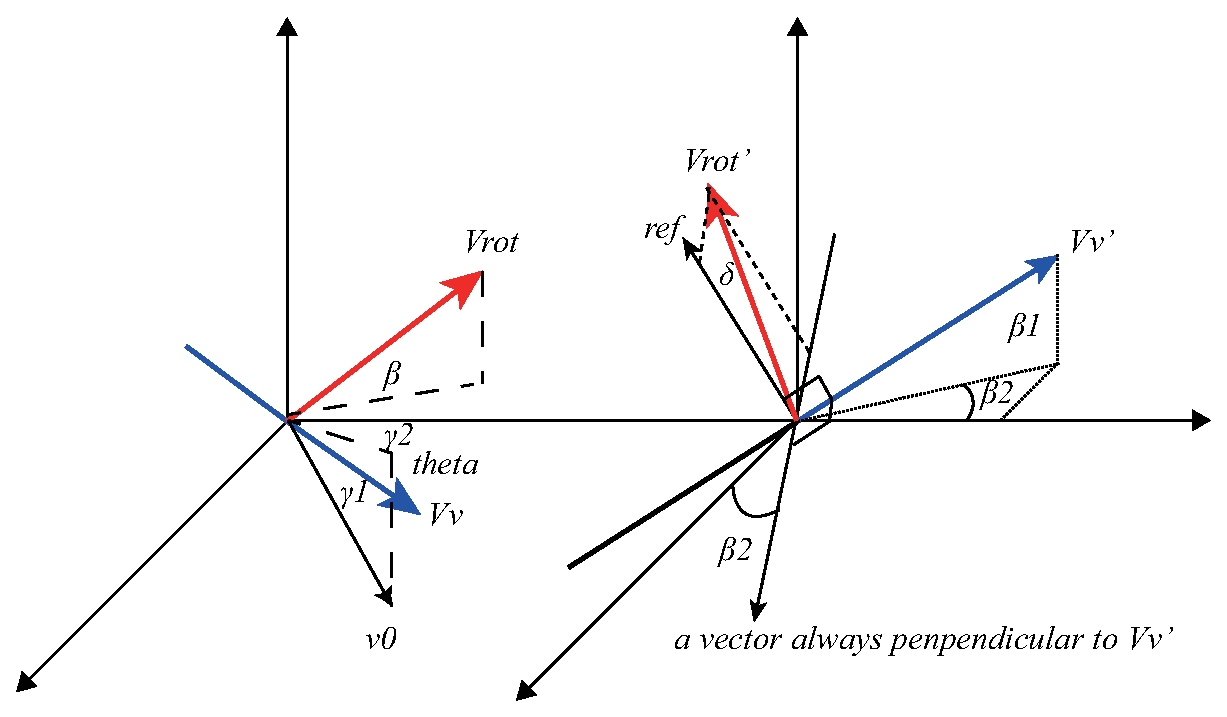
\includegraphics[width=0.7\textwidth]{geom}
	\caption{Collision geometry}
\end{figure}

Assume a collision between diatom($ N_1N_2$ ) and diatom($ N_3N_4 $), $N_2$ and $N_3$ are the atoms which collide. A body fitted right-hand-side coordinate system is formulated by unit vectors:
\begin{equation}
\begin{aligned}
\hat{v_x'} &= \begin{bmatrix}
\cos \beta_2, & \sin \beta_2, & 0
\end{bmatrix}^T  \\
\hat{v_v'} &= \begin{bmatrix}
-\cos \beta_1 \sin \beta_2, & \cos \beta_1 \cos \beta_2, & \sin \beta_1
\end{bmatrix}^T  \\
\hat{v_{ref}'} &= \begin{bmatrix}
\cos \beta_2, & \sin \beta_2, & 0 
\end{bmatrix}^T \times \hat{v_v'} = \begin{bmatrix}
\sin \beta_1 \sin \beta_2, & - \sin \beta_1 \cos \beta_2, & \cos \beta_1
\end{bmatrix} 
\end{aligned}
\end{equation}


Two rotational operation can transform the coordinates from original coordinates to the new one:
\begin{equation}
\begin{aligned}
\begin{bmatrix}
x' \\ y' \\z' 
\end{bmatrix}  = R_x (\beta_1) \cdot R_z(\beta_2) \begin{bmatrix}
x\\y\\z
\end{bmatrix}= \begin{bmatrix}
1 & 0 & 0 \\ 
0 & \cos \beta_1 & \sin \beta_1 \\ 
0 & -\sin \beta_1 & \cos \beta_1
\end{bmatrix} \cdot \begin{bmatrix} 
\cos \beta_2 & \sin \beta_2  & 0\\ 
-\sin \beta_2 & \cos \beta_2 & 0\\
0 & 0 &1
\end{bmatrix} \begin{bmatrix}
x\\y\\z
\end{bmatrix} 
\end{aligned}
\end{equation} 

Thus we can get:
\begin{equation}
\begin{bmatrix}
x\\y\\z
\end{bmatrix}  = R_z(-\beta_2) \cdot R_x(-\beta_1) \begin{bmatrix}
x' \\ y' \\z' 
\end{bmatrix} = \begin{bmatrix}
\cos \beta _2 & -\cos \beta _1 \sin \beta _2 & \sin
\beta _1 \sin \beta _2 \\
\sin \beta _2 & \cos \beta _1 \cos \beta _2 & -\cos
\beta _2 \sin \beta _1 \\
0 & \sin \beta _1 & \cos \beta _1 \\
\end{bmatrix}\begin{bmatrix}
x' \\ y' \\z' 
\end{bmatrix}  = A \begin{bmatrix}
x' \\ y' \\z' 
\end{bmatrix}  
\end{equation}

Then we have:
\begin{equation}
\begin{aligned}
\hat{v_v'} &= A \rvec{0}{1}{0} \\
\hat{v_{ref}'} & = A \rvec{0}{0}{1}  \\
\hat{v_r'} & = A \rvec{-\sin \delta}{0}{\cos \delta}= \begin{bmatrix}
-\cos \beta_2 \sin \delta +\sin \beta_1 \sin \beta_2 \cos \delta  \\
-\sin \beta_2 \sin \delta -\sin \beta_1 \cos \beta_2 \cos \delta  \\
\cos \beta_1 \cos \delta 
\end{bmatrix}
\end{aligned}
\end{equation}


Velocity vector for diatom($ N_1N_2$ )-diatom($ N_3N_4 $) collision:
\begin{equation}
\vec{v_2}^T =     \begin{bmatrix}
-\cos \beta \cos \theta & \sin \theta & \cos \gamma_1 \sin \gamma_2  \\ 
\cos \beta \sin \theta & \cos \theta & \cos \gamma_1 \cos \gamma_2  \\ 
\sin \beta & 0 & -\sin \gamma_1  
\end{bmatrix}  \begin{bmatrix}
   v_{r} \\
   v_v\\
   v
\end{bmatrix}
\end{equation}

\begin{equation}
\vec{v_3}^T =     \begin{bmatrix}
-\cos \beta_2 \sin \delta +\sin \beta_1 \sin \beta_2 \cos \delta  & -\cos \beta_1 \sin \beta_2 & -\cos \gamma_1 \sin \gamma_2 \\
-\sin \beta_2 \sin \delta -\sin \beta_1 \cos \beta_2 \cos \delta  & \cos \beta_1 \cos \beta_2 & - \cos \gamma_1 \cos \gamma_2 \\
\cos \beta_1 \cos \delta   & \sin \beta_1 & \sin \gamma_1  \\
\end{bmatrix}  \begin{bmatrix}
v_{r}' \\
v_v'\\
\dfrac{m}{M}v
\end{bmatrix}
\end{equation}

Pre-collision component of velocity on $ y-axis $:
\begin{equation}
\begin{aligned}
{v_2}_y &= v \cos \gamma _1 \cos \gamma _2+ v_r \cos \beta  \sin \theta +v_v \cos \theta\\
{v_3}_y &=-\frac{m }{M} v \cos \gamma _1 \cos \gamma_2 -  v_r'\left(\sin \beta _1 \cos\beta_2\cos \delta + \sin\beta_2\sin \delta \right)+ v_v' \cos \beta _1 \cos\beta _2
\end{aligned}
\end{equation}

The minimum velocity $ v $ to make post-vibrational energy equal to $ D $:
\begin{equation}
\begin{aligned}
v = \dfrac{1}{\cos \gamma_1 \cos \gamma_2}& \left[\dfrac{1}{\cos \theta} \left( \dfrac{\sqrt{D- m v_0^2 \sin^2 \phi_0} }{\sqrt{m}} + \dfrac{m+M\sin^2 \theta}{M+m} v_0 \cos \phi_0   \right)  \right.\\
& -\left. \dfrac{M}{m+M} \left(v_r'\left(\sin \beta _1 \cos\beta_2\cos \delta + \sin\beta_2\sin \delta \right)- v_1 \cos \phi_1 \cos \beta _1 \cos\beta _2 \right) \right. \\
& -\left. \dfrac{M}{m+M} \left(v_r \cos \beta \sin \theta \right) \right]
\end{aligned}
\end{equation}

Noted that the following term is the projection of velocity on y axis:
\begin{equation}
\boxed{
v_r'\left(\sin \beta _1 \cos\beta_2\cos \delta + \sin\beta_2\sin \delta\right)- v_1 \cos \phi_1 \cos \beta _1 \cos\beta _2}
\end{equation}

Then we can get the threshold $ E_t = \dfrac{2}{\mu} (mv)^2 $:
\begin{equation}
\begin{aligned}
E_t = \dfrac{2m^2/\mu}{\cos^2 \gamma_1 \cos^2 \gamma_2}& \left[\dfrac{M}{(m+M) \sqrt{m}} \left( \dfrac{\sqrt{D- E_v \sin^2 \phi_0} + \sqrt{E_v} \cos \phi_0 }{\cos \theta (M/(m+M))} - \sqrt{E_v} \cos\phi_0 \cos \theta - \sqrt{E_r} \cos\beta \sin \theta \right)  \right.\\
& -\left. \dfrac{\sqrt{M}}{m+M} \left( \sqrt{E_r'}\left( \cos \delta \cos\beta_2 \sin \beta _1  + \sin\beta_2\sin \delta \right)- \sqrt{E_v'}  \cos \phi_1 \cos \beta _1 \cos\beta _2 \right) \right]^2
\end{aligned}
\end{equation}



Again, define $ \alpha = (m/(M+m))^2 $, then we have:
\begin{gather}
\dfrac{m}{M+m} = \sqrt{\alpha}; \; \dfrac{M}{M+m} = 1-\sqrt{\alpha} \\
\dfrac{m}{M} = \dfrac{\sqrt{\alpha}}{1-\sqrt{\alpha}}; \;\dfrac{M}{m} = \dfrac{1-\sqrt{\alpha}}{\sqrt{\alpha}};
\end{gather}

Then:
\begin{equation}
\begin{aligned}
E_t = \dfrac{1 - \sqrt{\alpha}}{\cos^2 \gamma_1 \cos^2 \gamma_2}& \left[ \dfrac{\sqrt{D- E_v \sin^2 \phi_0} + \sqrt{E_v} \cos \phi_0 }{\cos \theta (1 - \sqrt{\alpha})} - \sqrt{E_v} \cos\phi_0 \cos \theta - \sqrt{E_r} \cos\beta \sin \theta \right.\\
& -\left.   \left(\dfrac{\sqrt{\alpha}}{1-\sqrt{\alpha}}\right)^{1/2}\left( \sqrt{E_r'}\left( \cos \delta \cos\beta_2 \sin \beta _1  + \sin\beta_2\sin \delta \right)- \sqrt{E_v'}  \cos \phi_1 \cos \beta _1 \cos\beta _2 \right) \right]^2
\end{aligned}
\end{equation}

Again, we use $ D_{eff} = D-E_r+ \dfrac{2E_r^{3/2}}{3(3bD)^{1/2}}$ to replace $ E_r $
\begin{equation}
\boxed{
\begin{aligned}
E_t = \dfrac{1 - \sqrt{\alpha}}{\cos^2 \gamma_1 \cos^2 \gamma_2}& \left[ \dfrac{\sqrt{D_{eff}- E_v \sin^2 \phi_0} + \sqrt{E_v} \cos \phi_0 }{\cos \theta (1 - \sqrt{\alpha})} - \sqrt{E_v} \cos\phi_0 \cos \theta \right.\\
& -\left.   \left(\dfrac{\sqrt{\alpha}}{1-\sqrt{\alpha}}\right)^{1/2}\left( \sqrt{E_r'}\left( \cos \delta \cos\beta_2 \sin \beta _1  + \sin\beta_2\sin \delta \right) \highlight{-} \sqrt{E_v'}  \cos \phi_1 \cos \beta _1 \cos\beta _2 \right) \right]^2
\end{aligned}}
\label{eq:1}
\end{equation}

The term $\left[\cos \delta \cos\beta_2 \sin \beta _1  + \sin\beta_2\sin \delta\right]$ can be replaced by $ \cos \alpha_1 \cos \alpha_2 $, in which $ \alpha_1 $  and  $ \alpha_2 $ are azimuth and polar angle for $ \vec{v_r'} $ 


The original one in the paper:
\begin{equation}
\boxed{
	\begin{aligned}
	E_t = \dfrac{1 - \sqrt{\alpha}}{\cos^2 \gamma_1 \cos^2 \gamma_2}& \left[ \dfrac{\sqrt{D_{eff}- E_v \sin^2 \phi_0} + \sqrt{E_v} \cos \phi_0 }{\cos \theta (1 - \sqrt{\alpha})} - \sqrt{E_v} \cos\phi_0 \cos \theta \right.\\
	& -\left.   \left(\dfrac{\sqrt{\alpha}}{1-\sqrt{\alpha}}\right)^{1/2}\left( \sqrt{E_r'}\left( \cos \delta \cos\beta_2 \sin \beta _1  + \sin\beta_2\sin \delta \right) \highlight{+}  \sqrt{E_v'}  \cos \phi_1 \cos \beta _1 \cos\beta _2 \right) \right]^2
	\end{aligned}}
\end{equation}

Optimum configuration and threshold function are same as the ones in original paper.
\begin{equation}
\begin{gathered}
\gamma_1 = \gamma_2 = \theta = \beta_1 = \phi_1 =0; \quad \delta = \dfrac{\pi}{2}; \quad \beta_2 = \pi - \arctan(\sqrt{E_r'/E_v'})
\end{gathered}
\end{equation}

\section{DSMC recipe}

There are 8 angles to be sampled. The range of sampling are:
\begin{equation}
\begin{aligned}
\text{Phase angle}:&\; \phi_0, \phi_1\in [0,2\pi]  \\
\text{Polar angle}:&\; \gamma_2, \beta_2 \in [0,2\pi]  \\
\text{Azimuth angle}:&\; \gamma_1, \beta_1 \in [0,\pi]  \\
\text{Reference angle}:&\; \theta, \delta \in [0,2\pi] 
\end{aligned}
\end{equation}


The region can be reduced by considering terms in Eq. \ref{eq:1}. 

First, the phase angles only appear in $ \sin^2\phi $ or $ \cos \phi $, thus:
\begin{align}
\text{Phase angle}:&\; \phi_0, \phi_1\in [0,\pi]  
\end{align}

Next, polar angle $ \gamma_2 $ appears as $ \cos^2\gamma_2 $. The reason is that only projection of velocity influences, thus $ \gamma_2 \in [0,\pi] $ has no difference compared to  $ \gamma_2 \in [\pi,2\pi] $
\begin{align}
\text{Polar angle}:&\; \gamma_2\in [0,\pi]  
\end{align}

Next, if we expand Eq. \ref{eq:1}, we will find that $ \theta $ only appears in $ \cos \theta, \cos^2 \theta, \cos^3 \theta, \cos^4 \theta $. Thus
In summary:
\begin{equation}
\boxed{
\begin{aligned}
& \phi_0, \phi_1, \gamma_2, \beta_1, \gamma_1 \in [0,\pi]  \\
& \beta_2, \theta, \delta \in [0,2\pi]  
\end{aligned}}
\end{equation}

\section{Matlab recipe}
We can also obtain the same results by Monte-Carlo sampling in Matlab. 
%\begin{algorithm}
%	\begin{algorithmic}[1]
%		\FOR{$i=0$ to $10$}
%		\STATE carry out some processing
%		\ENDFOR
%%		\FOR{$ e_v $  $ E_v(0) $ to $ E_v{end} $}
%%		\ENDFOR
%	\end{algorithmic}
%\end{algorithm}
\newpage
\begin{algorithm}
	\begin{algorithmic}[1]
		\For{$ E_v $ = $ E_v(0),...,E_v(end) $}
		    \State Sample $ E_t $ from $ f(\dfrac{E_t}{T}) =\dfrac{1}{\Gamma[5/2-\bar{\omega}]} \left(\dfrac{E_t}{T}\right)^{3/2-\bar{\omega}} \exp(-\dfrac{E_t}{T})  $
		    \State Sample $ E_r,E_r' $ from $ f(\dfrac{E_r}{T}) = \exp(-\dfrac{E_r}{T}) $
		    \State Sample $E_v'$ from $ P(E_v') = \dfrac{\exp(-E_v'/T_v)}{\sum_{j} \exp(-E_v'(j)/kT_v)} $
		    \State Sample angles
		    \State Calculate reaction probability $ P(v) $
		\EndFor
		\State Calculate VHS collision rates $ k_{coll}(T) $
		\State Reaction rates $ k(T,T_v) = k_{coll}(T) \dfrac{\sum_{j}P(j)\exp(-E_v(j)/T_v) }{\sum_{j} \exp(-E_v(j)/kT_v)} $
	\end{algorithmic}
\end{algorithm}

This method is much faster than DSMC (2 min v.s. 2 hours). It can also obtain rates for extreme low temperature since vibrational state-specific rates are directly calculated with the method. 
 \newpage
Appendix:

1. Volume  1 
\begin{gather}
\sum_{i=1}^{n} \left(\dfrac{x}{R_i} \right)^2 = 1\\
V = \dfrac{\Pi^{n/2} \prod_i R_i }{\Gamma[n/2 +1]} 
\end{gather}

2. Volume 2
\begin{gather}
\sum_{i=1}^{n-1} \left(\dfrac{x}{R_i} \right)^2 + \left(\dfrac{x}{R_n}\right)^4 = 1 \\
V = \dfrac{2 \pi ^{n/2-1} \Gamma[\dfrac{5}{4}] }{\Gamma \left[\dfrac{3}{4} + \dfrac{n}{2}\right]}\prod_i R_i 
\end{gather}

\end{document}